\documentclass[11pt]{article}
\usepackage[margin=2.6cm]{geometry}
\usepackage{graphicx,booktabs,amsmath,xcolor}
\usepackage[colorlinks=true,linkcolor=blue!50!black,citecolor=blue!50!black,urlcolor=blue!50!black]{hyperref}
\usepackage{caption}
\captionsetup{font=small,labelfont=bf,justification=justified}
\newcommand{\pt}{\ensuremath{p_\mathrm{T}}}
\graphicspath{{figures/}}

\title{\vspace{-1.2cm}{\color{red!70!black}\small\bfseries INTERNAL DRAFT --- UTA DFM GROUP --- NOT AN OFFICIAL ATLAS DOCUMENT}\\[2mm]
\Large Flavor-Dependent Machine-Learned Jet Calibration\\[1mm]
\normalsize DFM-NOTE-2026-02}
\author{\small UTA Detector Foundation Model group\\
\small (A.~Farbin, M.~A.~Ghaznavi, U.~Ghaznavi et al.; analysis assisted by Claude)}
\date{\small August 2026 \;\textbullet\; \texttt{github.com/afarbin/DetectorFoundationModel}, branch \texttt{dfm-merge}}

\begin{document}
\maketitle

\begin{abstract}
Extending the machine-learned jet \pt{} calibration of DFM-NOTE-2026-01 to
heavy-flavor jets, we rebuild the per-jet dataset with all flavors (1.20M matched
jets: ${\sim}850$k light, 150k $c$, 556k $b$, hadron-cone labels) and compare three
calibration strategies on the best backbone of Note~01: a flavor-blind shared model,
a flavor-conditioned shared model (truth-flavor one-hot into the head), and dedicated
per-flavor models. The uncorrected response differs by flavor as expected (light
$+4.4\%$ at 65--90\,GeV; $b$ on-scale with narrower core in $t\bar t$). Dedicated
per-flavor models lose clearly to the shared model for $c$ (JER 0.154 vs 0.131) and
$b$ (0.138 vs 0.128): cross-flavor statistics outweigh specialization at these sample
sizes. Flavor conditioning is the best strategy overall (best closure, 3.9\% RMS;
improves $b$), but presumes flavor knowledge at inference---directly motivating the
joint tagging--calibration architecture of DFM-NOTE-2026-03. The $b$-jet corrected
response exhibits the expected semileptonic low-side shoulder rather than a resolved
second mode.
\end{abstract}

\section{Introduction}
DFM-NOTE-2026-01~\cite{note1} established machine-learned jet \pt{} calibration on
light jets, halving the resolution of the input reconstruction with a
tracks + jet-features + cells model (TJC-graph). Jet response is, however,
flavor-dependent: $b$ and $c$ jets differ in shower composition, and semileptonic
heavy-flavor decays lose neutrino energy---a known pain point of classical calibration
chains. This note answers a practical question: given finite samples, should
heavy-flavor jets be calibrated by dedicated models, a shared model, or a shared model
conditioned on flavor? All dataset machinery, cuts, metrics, and the TJC-graph
backbone are as in Ref.~\cite{note1}, Sections~3--4; only the flavor selection
changes.

\section{Dataset}
The builder retains all truth-matched jets with hadron-cone labels in $\{0,4,5\}$
(light/$c$/$b$; taus excluded), storing the label per jet: 1{,}197{,}615 jets over
the 17 files---approximately 850k light, 150k $c$, 556k $b$ matched jets before
isolation ($t\bar t$ is $b$-rich by construction). Splits, quality cuts, isolation
flags, and spectrum weights are identical to Ref.~\cite{note1}.

\section{Strategies and results}
\begin{figure}[htbp]\centering
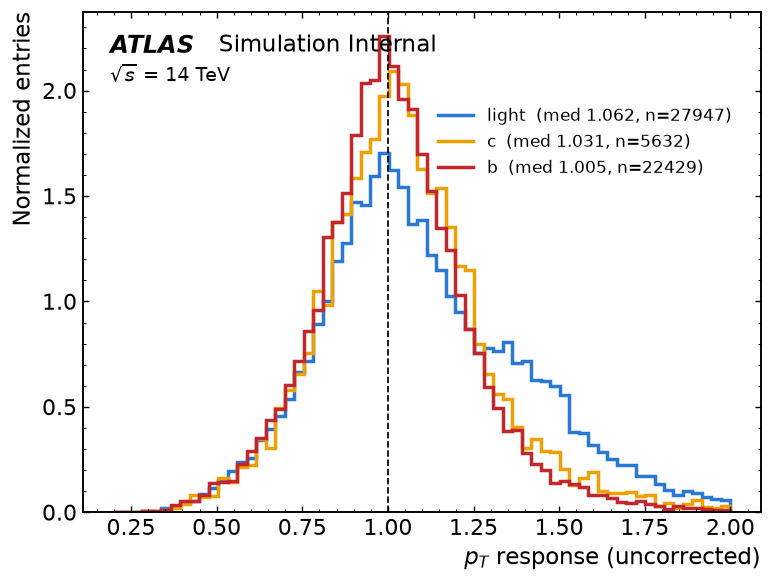
\includegraphics[width=0.62\textwidth]{FP1_uncorr_flavor.png}
\caption{Uncorrected \pt{} response by flavor (isolated test jets): light jets read
$+4.4\%$ high at 65--90\,GeV; $b$ jets are on-scale with a narrower core---in
$t\bar t$ the semileptonic deficit is partly offset by $b$ jets being harder and more
central. The shape differences are what a flavor-aware calibration exploits.}
\label{fig:uncorr}
\end{figure}

\begin{table}[htbp]\centering\small
\begin{tabular}{lcccc}\toprule
evaluated on & uncorrected & blind shared & flavor-conditioned & dedicated\\\midrule
light JER@65--90 & 0.230 & 0.1152 & \textbf{0.1150} & 0.1152\\
$c$ JER@65--90 & 0.182 & \textbf{0.1305} & 0.1328 & 0.1536\\
$b$ JER@65--90 & 0.176 & 0.1305 & \textbf{0.1283} & 0.1384\\
overall closure RMS & --- & 4.3\% & \textbf{3.9\%} & ---\\\bottomrule
\end{tabular}
\caption{JER at 65--90\,GeV per flavor under the three strategies (TJC-graph
backbone, 3 seeds).}
\label{tab:strat}
\end{table}

\begin{figure}[htbp]\centering
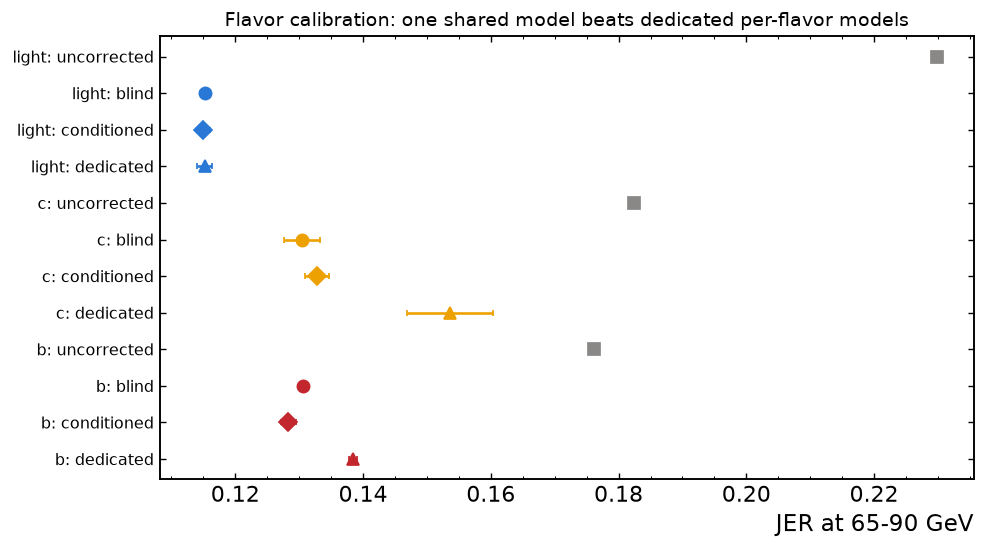
\includegraphics[width=0.72\textwidth]{FP2_jer_matrix.png}
\caption{JER at 65--90\,GeV, flavor $\times$ strategy: squares = uncorrected,
circles = blind shared, diamonds = truth-flavor conditioned, triangles = dedicated.
Dedicated models are visibly worse for $c$ and $b$.}
\label{fig:matrix}
\end{figure}
\begin{figure}[htbp]\centering
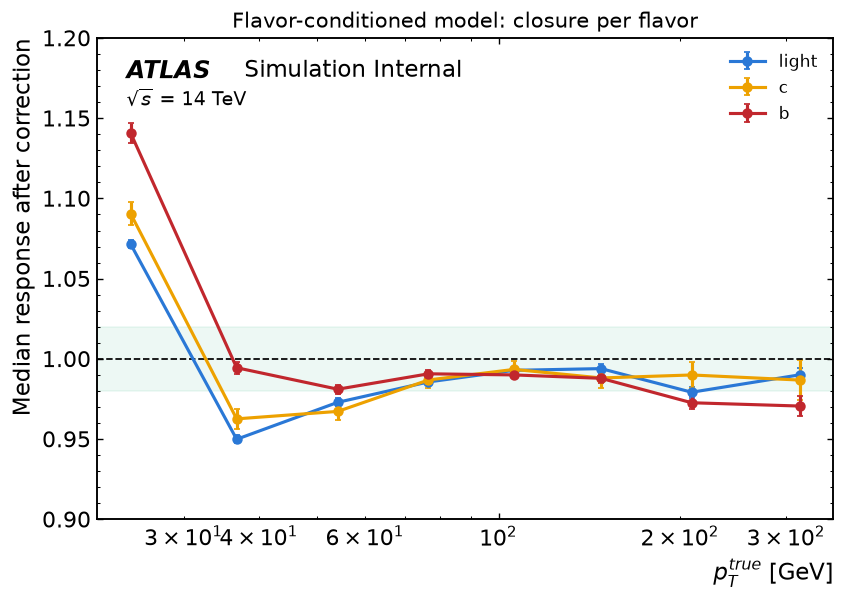
\includegraphics[width=0.66\textwidth]{FP3_closure_flavor.png}
\caption{Flavor-conditioned model: closure per flavor within ${\sim}2\%$ above
45\,GeV; the shared low-\pt{} non-closure of Note~01 remains.}
\label{fig:closure}
\end{figure}
\begin{figure}[htbp]\centering
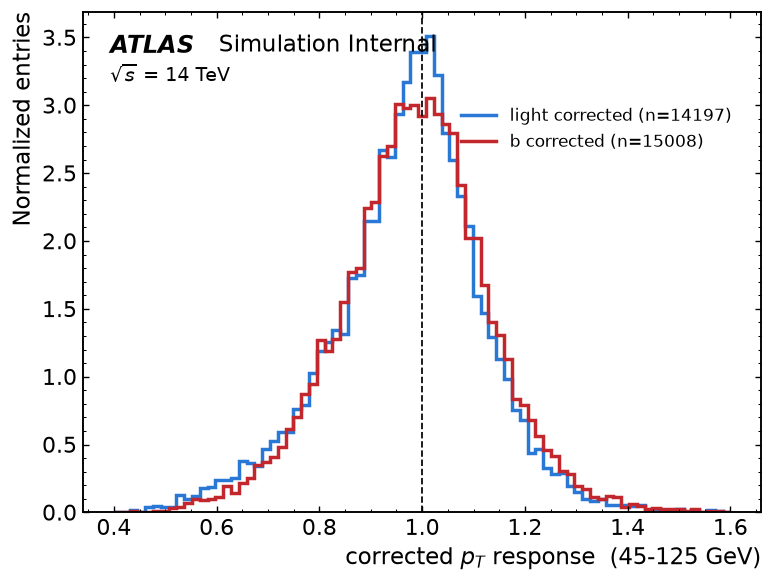
\includegraphics[width=0.62\textwidth]{FP4_b_bimodality.png}
\caption{Corrected $b$-jet response versus light at 45--125\,GeV: a broadened
low-side shoulder from semileptonic decays rather than a resolved second mode; a
single Gaussian per-jet $\sigma$ remains defensible, with a mixture-density head as
the identified upgrade path.}
\label{fig:bimodal}
\end{figure}

\section{Conclusions}
\textbf{One shared model beats separate calibrations} at these statistics: dedicated
$c$ and $b$ models are starved of data relative to what cross-flavor sharing
provides. \textbf{Flavor conditioning is the best overall strategy}---matching the
blind model for light and $c$ while improving $b$ and overall closure---but requires
flavor knowledge at inference. The natural resolution is to predict flavor and
calibration jointly, which is the subject of DFM-NOTE-2026-03~\cite{note3}.

\begin{thebibliography}{9}
\bibitem{note1} DFM-NOTE-2026-01, \emph{Machine-Learned Jet \pt{} Calibration from
Low-Level Detector Information},
\texttt{notes/DFM-NOTE-2026-01-jet-pt-calibration/}.
\bibitem{note3} DFM-NOTE-2026-03, \emph{Panoptic Flavor Tagging and Jet Calibration},
\texttt{notes/DFM-NOTE-2026-03-panoptic-tagging-calibration/}.
\end{thebibliography}
\end{document}
